\documentclass[UTF8,fontset=fandol,zihao=-4,a4paper]{ctexart}
\usepackage[left=25mm,right=25mm,top=24mm,bottom=24mm]{geometry}
\usepackage{amsmath,amssymb,amsthm,mathtools}
\usepackage{fontspec}
\setmainfont{XITS}
\usepackage{graphicx,booktabs,array,longtable}
\usepackage{tikz,pgfplots}
\pgfplotsset{compat=1.18}
\usetikzlibrary{arrows.meta,positioning}
\usepackage{enumitem}
\usepackage[font=small,labelfont=bf,labelsep=quad]{caption}
\usepackage[hidelinks,unicode]{hyperref}
\usepackage{bookmark}
\usepackage{setspace}
\setstretch{1.18}
\pagestyle{plain}
\setlength{\parskip}{2.5pt}
\setlength{\emergencystretch}{1.5em}
\setlength{\abovedisplayskip}{8pt plus 2pt minus 2pt}
\setlength{\belowdisplayskip}{8pt plus 2pt minus 2pt}
\setlength{\textfloatsep}{15pt}
\setlength{\intextsep}{14pt}
\ctexset{section={format=\Large\bfseries,beforeskip=18pt,afterskip=9pt},subsection={format=\large\bfseries,beforeskip=13pt,afterskip=6pt}}
\numberwithin{equation}{section}
\newtheoremstyle{reportplain}{8pt}{8pt}{\normalfont}{0pt}{\bfseries}{\quad}{0pt}{}
\theoremstyle{reportplain}
\newtheorem{theorem}{定理}[section]
\newtheorem{proposition}[theorem]{命题}
\newtheorem{lemma}[theorem]{引理}
\newtheorem{corollary}[theorem]{推论}
\newtheorem{definition}[theorem]{定义}
\newtheorem{remark}[theorem]{注}
\renewcommand{\proofname}{证明}
\renewcommand{\qedsymbol}{\ensuremath{\square}}
\newcommand{\Pow}{\mathcal P}
\newcommand{\muA}{\mu_A}
\newcommand{\ind}{\mathbf 1}
\newcommand{\cut}[1]{A_{#1}}
\newcommand{\scut}[1]{A_{#1}^{+}}
\newcommand{\set}[1]{\{#1\}}
\newcommand{\eqtag}[1]{\label{#1}}
\hypersetup{pdftitle={模糊集广义分解定理中的截集恢复及其有限重构},pdfsubject={系统数学专题报告},pdfkeywords={模糊集,截集,广义分解定理,集合族,有限重构}}
\begin{document}
\begin{center}
{\LARGE\bfseries 模糊集广义分解定理中的\par 截集恢复及其有限重构\par}
\vspace{9pt}
{\normalsize 系统数学专题报告}\par
\vspace{6pt}
{\small 2026 年 10 月}
\end{center}
\vspace{5pt}
\noindent\textbf{摘要}\quad
模糊集的普通截集与强截集仅在临界隶属度处存在差异。广义分解定理允许集合值映射在二者之间自由选择，却仍能通过严格位于目标阈值两侧的集合族恢复确定的截集。本文围绕课程定理 3.7 的第（3）条，给出两种恢复式的逐元素双向包含证明，明确交集中的全称量词与并集中的存在量词，并利用中点构造消除边界选择的不确定性。在此基础上，讨论集合族单调性、隶属函数重构、稠密阈值替代与单侧序列表示；针对有限隶属度值集，给出中点见证的有限证书和单阈值精确重构方法。四元素教学实例与六元素课程实例说明，改变临界层的合法选择不会改变恢复结果。最后分析空索引族端点、有限采样的逻辑局限及离散计算的精确性。结论表明，截集恢复依赖于隶属度区间的序结构与严格分离，而不依赖于隶属函数的连续性或临界元素的具体选取。

\vspace{5pt}
\noindent\textbf{关键词}\quad 模糊集；普通截集；强截集；广义分解定理；中点见证；有限重构

\vspace{10pt}
\noindent\textbf{Abstract}\quad
Ordinary and strong cuts of a fuzzy set differ only at elements whose membership grades coincide with the cut level. The generalized decomposition theorem permits a set-valued family to choose these boundary elements freely while retaining exact recovery of both cuts. This report presents elementwise proofs of the two recovery identities, emphasizing universal and existential quantification and strict midpoint witnesses. It then derives monotonicity, membership reconstruction, dense-level recovery and one-sided sequential representations. For a finite set of membership grades, finite witness certificates and exact single-level reconstruction are established. A four-element teaching example and a six-element course example illustrate invariance under legal boundary choices. Endpoint conventions, the limitations of finite sampling and exact discrete arithmetic are also examined. The results depend on the order structure of the membership interval rather than continuity of the membership function.

\noindent\textbf{Keywords}\quad fuzzy sets; cut recovery; generalized decomposition; midpoint witnesses; finite reconstruction

\section{引言}
经典集合以属于或不属于两种状态刻画元素。模糊集则允许元素具有介于 0 与 1 之间的隶属度，从而描述具有渐变边界的概念。Zadeh 的奠基性工作以隶属函数定义模糊集，并将包含、并、交等基本运算推广到模糊情形\cite{zadeh}。截集提供了连接模糊集合与清晰集合的基本方式：给定一个阈值，将隶属度达到该阈值的元素组成普通集合。相关表示方法是模糊集理论的基础内容\cite{klir,zimmermann}。

在截集表示中，普通截集采用大于等于关系，强截集采用严格大于关系。当若干元素的隶属度恰好等于阈值时，二者可能不同。课程中的广义分解定理进一步考虑集合值映射 $H$：每个高度处的 $H$ 可以在强截集与普通截集之间选择。问题在于，这些边界选择是否使原有截集信息丢失，以及为何对一侧集合族取交或取并仍能精确恢复。

本文对应《第3章 模糊向清晰的转换》第 35 页定理 3.7，第 37 页相关证明及第 41 页例 3.1\cite{course}，重点分析第（3）条。第（1）、（2）条用于说明隶属函数重构与集合族单调性之间的联系。本文属于经典定理的专题论证与补充推导，有限重构结论用于解释数值验证，并不将课程中的既有定理作为新的研究成果。

全文的论证路线为：首先建立统一的截集记号与边界分解；其次证明两种恢复式，并说明严格索引条件的必要性；随后给出单调集合族的表示、稠密阈值与序列形式；最后讨论有限重构、具体实例、计算验证及适用边界。所有核心证明均在一般论域上成立，数值结果用于核对结论，而不是替代证明。

\section{基本定义与边界结构}
\subsection{模糊集与两种截集}
设 $X$ 为非空论域，$\Pow(X)$ 为其幂集。论域上的模糊集 $A$ 由隶属函数
\begin{equation}
\muA:X\longrightarrow[0,1]
\eqtag{eq:membership}
\end{equation}
确定。本文不要求 $X$ 带有拓扑结构，也不要求 $\muA$ 连续。字母 $\lambda$ 表示需要恢复的目标高度，$\alpha$ 表示用于恢复的索引高度，两者的取值均属于 $[0,1]$。

\begin{definition}[普通截集与强截集]
对任意 $\lambda\in[0,1]$，定义
\begin{align}
\cut{\lambda}&=\set{x\in X:\muA(x)\ge\lambda},\eqtag{eq:ordinary}\\
\scut{\lambda}&=\set{x\in X:\muA(x)>\lambda}.\eqtag{eq:strong}
\end{align}
上标 $+$ 表示强截集，不表示加法或集合的正部。
\end{definition}

记临界等值层为 $E_\lambda=\set{x\in X:\muA(x)=\lambda}$。由定义立即得到不交分解
\begin{equation}
\cut{\lambda}=\scut{\lambda}\mathbin{\dot\cup}E_\lambda.
\eqtag{eq:boundary}
\end{equation}
因此，两种截集的差集恰好为 $E_\lambda$。当没有元素的隶属度等于 $\lambda$ 时，普通截集与强截集相同；当等值层非空时，是否保留这一层决定了二者的差异。

连续教学曲线 $\muA(x)=1-|x-2|/2$，$X=[0,4]$，给出直观例子：对 $0\le\lambda<1$，普通截集为 $[2\lambda,4-2\lambda]$，强截集为 $(2\lambda,4-2\lambda)$；当 $\lambda=1$ 时，普通截集为单点集 $\set{2}$，强截集为空集。图~\ref{fig:cuts} 中取 $\lambda=0.60$，边界横坐标分别为 1.20 和 2.80。

\begin{figure}[htbp]
\centering
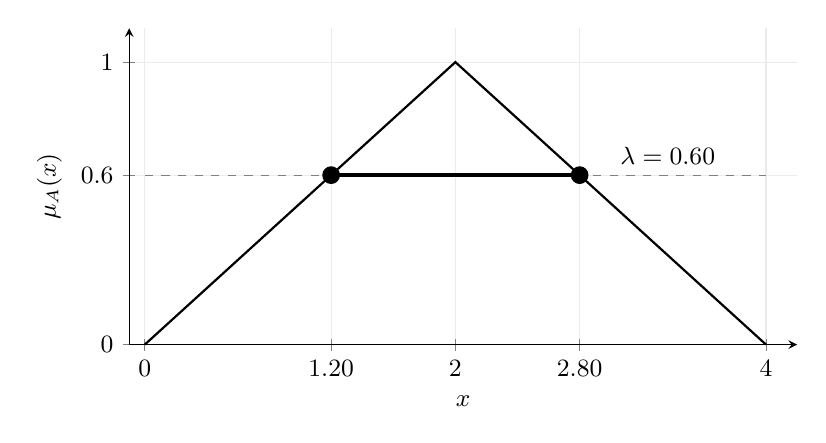
\begin{tikzpicture}
\begin{axis}[width=.83\textwidth,height=5.6cm,xmin=-.1,xmax=4.2,ymin=0,ymax=1.12,axis lines=left,xlabel={$x$},ylabel={$\mu_A(x)$},xtick={0,1.2,2,2.8,4},xticklabels={$0$,$1.20$,$2$,$2.80$,$4$},ytick={0,.6,1},grid=major,grid style={gray!16},tick label style={font=\small},label style={font=\small},clip=false]
\addplot[thick,black] coordinates {(0,0)(2,1)(4,0)};
\addplot[dashed,gray] coordinates {(0,.6)(4,.6)};
\addplot[very thick] coordinates {(1.2,.6)(2.8,.6)};
\addplot[only marks,mark=*,mark size=3pt] coordinates {(1.2,.6)(2.8,.6)};
\node[anchor=west,font=\small] at (axis cs:3,.67) {$\lambda=0.60$};
\end{axis}
\end{tikzpicture}
\caption{三角形隶属函数的水平截集。实心端点对应普通截集；将端点改为空心即可表示强截集。}
\label{fig:cuts}
\end{figure}

\subsection{合法集合族与可选边界}
\begin{definition}[夹逼集合族]
若集合值映射 $H:[0,1]\to\Pow(X)$ 满足
\begin{equation}
\scut{\alpha}\subseteq H(\alpha)\subseteq\cut{\alpha},
\qquad\forall\alpha\in[0,1],
\eqtag{eq:sandwich}
\end{equation}
则称 $H$ 为关于 $A$ 的合法夹逼集合族。
\end{definition}

对固定的 $\alpha$，式~\eqref{eq:sandwich} 等价于以下成员规则：若 $\muA(x)>\alpha$，则必须有 $x\in H(\alpha)$；若 $\muA(x)<\alpha$，则必须有 $x\notin H(\alpha)$；若 $\muA(x)=\alpha$，两种选择都合法。自由选择只发生在等值层，不能任意改变其他元素的成员资格。

\begin{proposition}[边界选择的完整参数化]
式~\eqref{eq:sandwich} 成立，当且仅当存在 $B_\alpha\subseteq E_\alpha$，使得
\begin{equation}
H(\alpha)=\scut{\alpha}\mathbin{\dot\cup}B_\alpha.
\eqtag{eq:parameter}
\end{equation}
\end{proposition}
\begin{proof}
若夹逼条件成立，取 $B_\alpha=H(\alpha)\setminus\scut{\alpha}$。由于 $H(\alpha)\subseteq\cut{\alpha}$，其与强截集的差集属于 $E_\alpha$，从而得到式~\eqref{eq:parameter}。反之，任何 $B_\alpha\subseteq E_\alpha$ 与强截集的不交并都包含强截集，并包含于普通截集。\end{proof}

\begin{lemma}[夹逼条件蕴含单调性]
对任意 $0\le\alpha<\beta\le1$，有 $H(\beta)\subseteq H(\alpha)$。
\end{lemma}
\begin{proof}
若 $x\in\cut{\beta}$，则 $\muA(x)\ge\beta>\alpha$，所以 $x\in\scut{\alpha}$。结合夹逼条件得到
\begin{equation}
H(\beta)\subseteq\cut{\beta}\subseteq\scut{\alpha}\subseteq H(\alpha).
\eqtag{eq:monotonic}
\end{equation}
\end{proof}
这说明 $H$ 随高度增加而递减。即使不同等值层的子集 $B_\alpha$ 分别选择，这种单调性仍自动成立，无须再额外假设。

\section{截集恢复定理与严格证明}
\subsection{定理陈述}
\begin{theorem}[截集恢复]
设 $A$ 为 $X$ 上的模糊集，$H$ 满足式~\eqref{eq:sandwich}。则
\begin{align}
\cut{\lambda}&=\bigcap_{\substack{\alpha\in[0,1]\\\alpha<\lambda}}H(\alpha),
&&0<\lambda\le1,\eqtag{eq:left}\\
\scut{\lambda}&=\bigcup_{\substack{\alpha\in[0,1]\\\alpha>\lambda}}H(\alpha),
&&0\le\lambda<1.\eqtag{eq:right}
\end{align}
\end{theorem}

式~\eqref{eq:left} 从目标高度下方取交，恢复普通截集；式~\eqref{eq:right} 从目标高度上方取并，恢复强截集。所有索引高度都限定在 $[0,1]$ 内，且两式均不包含 $\alpha=\lambda$。端点限制保证相应索引族非空，空族约定将在第~\ref{sec:endpoints} 节单独讨论。

\subsection{普通截集的两个包含方向}
\begin{proof}[式~\eqref{eq:left} 的证明]
记 $L_\lambda=\bigcap_{\alpha<\lambda}H(\alpha)$。

\textbf{第一步，证明 $\cut{\lambda}\subseteq L_\lambda$。} 任取 $x\in\cut{\lambda}$，则 $\muA(x)\ge\lambda$。对任意 $\alpha\in[0,\lambda)$，都有
\begin{equation}
\muA(x)\ge\lambda>\alpha.
\eqtag{eq:left-in}
\end{equation}
故 $x\in\scut{\alpha}\subseteq H(\alpha)$。由于这一判断对每个下方高度成立，$x$ 属于所有这些集合的交集，得到 $x\in L_\lambda$。

\textbf{第二步，证明 $L_\lambda\subseteq\cut{\lambda}$。} 采用逆否论证。若 $x\notin\cut{\lambda}$，则 $\muA(x)<\lambda$。令
\begin{equation}
\alpha_x=\frac{\muA(x)+\lambda}{2}.
\eqtag{eq:left-mid}
\end{equation}
因为 $0\le\muA(x)<\lambda\le1$，该中点是合法索引，并满足
\begin{equation}
\muA(x)<\alpha_x<\lambda.
\eqtag{eq:left-witness}
\end{equation}
于是 $x\notin\cut{\alpha_x}$。又因为 $H(\alpha_x)\subseteq\cut{\alpha_x}$，可知 $x\notin H(\alpha_x)$。至少一个下方集合排除了 $x$，故 $x\notin L_\lambda$。由逆否命题得到第二个包含关系，两者合并即得结论。
\end{proof}

这段证明揭示了普通截集保留临界元素的原因。若 $\muA(x)=\lambda$，虽然 $x$ 在 $H(\lambda)$ 中可选，但对于每个 $\alpha<\lambda$ 都有 $\muA(x)>\alpha$，因此它在所有参与求交的集合中都必须出现。

\subsection{强截集的两个包含方向}
\begin{proof}[式~\eqref{eq:right} 的证明]
记 $U_\lambda=\bigcup_{\alpha>\lambda}H(\alpha)$。

\textbf{第一步，证明 $\scut{\lambda}\subseteq U_\lambda$。} 任取 $x\in\scut{\lambda}$，有 $\muA(x)>\lambda$。令
\begin{equation}
\beta_x=\frac{\lambda+\muA(x)}2,
\qquad\lambda<\beta_x<\muA(x)\le1.
\eqtag{eq:right-mid}
\end{equation}
故 $x\in\scut{\beta_x}\subseteq H(\beta_x)$。存在一个上方集合包含 $x$，因而 $x\in U_\lambda$。

\textbf{第二步，证明 $U_\lambda\subseteq\scut{\lambda}$。} 任取 $x\in U_\lambda$。根据并集定义，存在 $\alpha\in(\lambda,1]$，使 $x\in H(\alpha)$。由 $H(\alpha)\subseteq\cut{\alpha}$ 得
\begin{equation}
\muA(x)\ge\alpha>\lambda,
\eqtag{eq:right-out}
\end{equation}
故 $x\in\scut{\lambda}$。合并两个包含关系即可完成证明。
\end{proof}

当 $\muA(x)=\lambda$ 时，每个 $\alpha>\lambda$ 都严格高于其隶属度，因此这些 $H(\alpha)$ 全部排除 $x$，它无法进入并集。普通截集和强截集的区别由索引的一侧性决定，而不是由 $H(\lambda)$ 的实际选择决定。

\subsection{量词结构与严格索引}
交集与并集分别对应如下逻辑条件：
\begin{align}
x\in\bigcap_{\alpha<\lambda}H(\alpha)
&\iff\forall\alpha<\lambda,\ x\in H(\alpha),\eqtag{eq:forall}\\
x\in\bigcup_{\alpha>\lambda}H(\alpha)
&\iff\exists\alpha>\lambda,\ x\in H(\alpha).\eqtag{eq:exists}
\end{align}
在普通式中，证明成员资格要检查全部下方高度，而排除成员只需找到一个反例高度；在强式中，确认成员只需找到一个上方见证，而排除成员要说明全部上方高度均不包含它。中点正是完成这些存在性步骤的统一构造。

\begin{proposition}[将严格索引改为非严格索引的结果]
对每个 $\lambda\in[0,1]$，有
\begin{equation}
\bigcap_{0\le\alpha\le\lambda}H(\alpha)=H(\lambda)
=\bigcup_{\lambda\le\alpha\le1}H(\alpha).
\eqtag{eq:inclusive}
\end{equation}
\end{proposition}
\begin{proof}
单调性表明 $H(\lambda)$ 包含于每个更低高度的集合；同时 $H(\lambda)$ 本身参与左侧求交，因此交集等于 $H(\lambda)$。对于右侧求并，每个更高高度的集合都包含于 $H(\lambda)$，而 $H(\lambda)$ 本身也参与求并，因此并集同样等于它。\end{proof}
所以，若将 $\alpha<\lambda$ 改成 $\alpha\le\lambda$，或将 $\alpha>\lambda$ 改成 $\alpha\ge\lambda$，所得结果一般只是任意选择的临界集合。严格索引是定理的一部分，而不是排版细节。

\section{集合族表示与稠密阈值重构}
\subsection{从集合族恢复隶属函数}
对于固定元素 $x$，定义其被包含的高度集合
\begin{equation}
S_x=\set{\alpha\in[0,1]:x\in H(\alpha)}.
\eqtag{eq:sx}
\end{equation}
由夹逼条件可知，若 $t=\muA(x)$，则 $[0,t)\subseteq S_x\subseteq[0,t]$。当 $t=0$ 时，$S_x$ 可以为空，也可以只包含 0。为统一处理端点，以下上确界均取于完备格 $[0,1]$，规定 $\sup_{[0,1]}\varnothing=0$。

\begin{corollary}[隶属度重构]
对任意 $x\in X$，有
\begin{equation}
\muA(x)=\sup_{[0,1]}S_x
=\sup_{\alpha\in[0,1]}\bigl[\alpha\ind_{H(\alpha)}(x)\bigr],
\eqtag{eq:resolution}
\end{equation}
其中 $\ind_C$ 为清晰集合 $C$ 的示性函数。
\end{corollary}
\begin{proof}
当 $t>0$ 时，所有严格小于 $t$ 的高度都包含 $x$，且任何包含 $x$ 的高度不超过 $t$，故 $\sup S_x=t$。当 $t=0$ 时，由约定仍有 $\sup S_x=0$。右式中被包含的高度贡献 $\alpha$，不被包含的高度贡献 0，因而与前式相同。\end{proof}

式~\eqref{eq:resolution} 以点值形式说明课程广义分解定理第（1）条：高度加权的清晰集合族，在逐点取上确界后重构原模糊集。边界是否取到最高高度不影响上确界，因此一般只保证上确界，不能将其无条件替换为最大值。

\begin{proposition}[递减集合族的等价表示]
若 $H:[0,1]\to\Pow(X)$ 随高度递减，则存在唯一的隶属函数 $\mu:X\to[0,1]$，使 $\set{x:\mu(x)>\alpha}\subseteq H(\alpha)\subseteq\set{x:\mu(x)\ge\alpha}$ 对所有 $\alpha$ 成立。该函数由 $\mu(x)=\sup_{[0,1]}S_x$ 给出。
\end{proposition}
\begin{proof}
若 $x\in H(\alpha)$，则 $\alpha\in S_x$，所以 $\mu(x)\ge\alpha$，得到上界。若 $\mu(x)>\alpha$，依据上确界定义，存在 $\beta\in S_x$ 满足 $\beta>\alpha$。于是 $x\in H(\beta)\subseteq H(\alpha)$，得到下界。唯一性由式~\eqref{eq:resolution} 的同样论证得到。\end{proof}

因此，夹逼集合族不仅保留全部截集，还确定唯一的隶属函数。这里的“唯一”指模糊集唯一；对于同一模糊集，临界子集 $B_\alpha$ 仍可能产生多个不同的合法 $H$。

\subsection{稠密阈值替代}
\begin{theorem}[稠密高度集合上的恢复]
设 $D\subseteq[0,1]$ 在 $[0,1]$ 中稠密。则在原定理的对应范围内，有
\begin{align}
\cut{\lambda}&=\bigcap_{\substack{\alpha\in D\\\alpha<\lambda}}H(\alpha),\eqtag{eq:dense-left}\\
\scut{\lambda}&=\bigcup_{\substack{\alpha\in D\\\alpha>\lambda}}H(\alpha).\eqtag{eq:dense-right}
\end{align}
\end{theorem}
\begin{proof}
普通式中，对 $\muA(x)\ge\lambda$ 的元素，下方任何高度都必须包含它。对 $\muA(x)<\lambda$ 的元素，稠密性保证开区间 $(\muA(x),\lambda)$ 内存在 $\alpha\in D$，该高度必定排除它。强式中，对 $\muA(x)>\lambda$ 的元素，开区间 $(\lambda,\muA(x))$ 内存在 $\alpha\in D$，该高度必定包含它；其余元素则在全部上方高度被排除。\end{proof}

特别地，可取 $D=\mathbb Q\cap[0,1]$。这表明对一般论域，可数稠密的高度集合已足够恢复截集。但可数无穷并不等于有限；将稠密集合截断为有限网格后，精确结论通常不能直接保留。

\subsection{单侧序列与集合意义的极限}
固定 $0<\lambda\le1$，取 $\alpha_n=\lambda(1-1/(n+1))$，则 $\alpha_n\uparrow\lambda$ 且 $\alpha_n<\lambda$。固定 $0\le\lambda<1$，取 $\beta_n=\lambda+(1-\lambda)/(n+1)$，则 $\beta_n\downarrow\lambda$ 且 $\beta_n>\lambda$。有
\begin{equation}
\cut{\lambda}=\bigcap_{n=1}^{\infty}H(\alpha_n),
\qquad
\scut{\lambda}=\bigcup_{n=1}^{\infty}H(\beta_n).
\eqtag{eq:sequence}
\end{equation}
例如，当 $\muA(x)<\lambda$ 时，随着 $\alpha_n$ 递增，最终必有 $\alpha_n>\muA(x)$，从而排除 $x$。另一式同理。这些序列只需从相应一侧逼近 $\lambda$，无需在整个区间稠密。

由于 $H(\alpha_n)$ 递减、$H(\beta_n)$ 递增，式~\eqref{eq:sequence} 可以看作单侧的集合极限。两侧结果的差集为 $E_\lambda$，而 $H(\lambda)$ 位于两侧结果之间。该结论不表示 $H$ 在 $\lambda$ 处连续，也不需要引入集合值映射的拓扑连续性。

\section{有限隶属度值集下的精确重构}
\subsection{逐元素中点见证证书}
设 $X=\set{x_1,\ldots,x_n}$，记 $m_i=\muA(x_i)$。对于固定目标高度，定义
\begin{align}
W^-_\lambda&=\set{(m_i+\lambda)/2:m_i<\lambda},\eqtag{eq:wminus}\\
W^+_\lambda&=\set{(\lambda+m_i)/2:m_i>\lambda}.\eqtag{eq:wplus}
\end{align}
重复的高度只保留一次。这两个集合分别为需要排除的元素和需要找回的元素提供见证。

\begin{proposition}[有限证书]
采用空交为 $X$、空并为空集的约定时，对任意 $\lambda\in[0,1]$，有
\begin{equation}
\cut{\lambda}=\bigcap_{\alpha\in W^-_\lambda}H(\alpha),
\qquad
\scut{\lambda}=\bigcup_{\alpha\in W^+_\lambda}H(\alpha).
\eqtag{eq:finite-certificate}
\end{equation}
\end{proposition}
\begin{proof}
普通式中，$\muA(x_i)\ge\lambda$ 的元素在所有 $W^-_\lambda$ 高度处均被包含；$\muA(x_i)<\lambda$ 的元素至少被其自身中点高度排除。若 $W^-_\lambda=\varnothing$，则全部元素满足 $\muA(x_i)\ge\lambda$，此时空交与普通截集都等于 $X$。强式中，每个高于 $\lambda$ 的元素在其自身中点高度被包含，其他元素在所有见证高度处均被排除；若 $W^+_\lambda=\varnothing$，则二者均为空集。\end{proof}

有限证书的正确性来自逐元素的严格分离。它并非声称任取有限个高度即可代替无限交或并，而是为每个相关元素构造了足以决定成员资格的高度。证书中部分高度可能恰好等于另一个元素的隶属度；该元素的边界选择仍不影响证书整体的正确性。

\subsection{单阈值重构与相邻高度间隙}
事实上，上述证书还能进一步压缩。当低于 $\lambda$ 的隶属度值非空时，令
\begin{equation}
m_- =\max\set{\muA(x):\muA(x)<\lambda},
\qquad\gamma_-=(m_-+\lambda)/2.
\eqtag{eq:lower-gap}
\end{equation}
当高于 $\lambda$ 的值非空时，令
\begin{equation}
m_+ =\min\set{\muA(x):\muA(x)>\lambda},
\qquad\gamma_+=(\lambda+m_+)/2.
\eqtag{eq:upper-gap}
\end{equation}

\begin{theorem}[有限值集的单阈值精确重构]
若 $\muA(X)$ 为有限集合，则对 $0<\lambda\le1$，存在 $\gamma_-<\lambda$ 使
\begin{equation}
H(\gamma_-)=\cut{\lambda};
\eqtag{eq:single-left}
\end{equation}
对 $0\le\lambda<1$，存在 $\gamma_+>\lambda$ 使
\begin{equation}
H(\gamma_+)=\scut{\lambda}.
\eqtag{eq:single-right}
\end{equation}
存在相邻值时，可分别采用式~\eqref{eq:lower-gap} 和式~\eqref{eq:upper-gap} 的中点；若没有低于 $\lambda$ 的值，可取 $\gamma_-=\lambda/2$；若没有高于 $\lambda$ 的值，可取 $\gamma_+=(\lambda+1)/2$。
\end{theorem}
\begin{proof}
先考虑普通式。若 $\muA(x)<\lambda$，则 $\muA(x)\le m_-<\gamma_-$，故 $H(\gamma_-)$ 必须排除 $x$；若 $\muA(x)\ge\lambda$，则 $\muA(x)\ge\lambda>\gamma_-$，故必须包含 $x$。因此成员资格与 $\cut{\lambda}$ 完全一致。若没有较低值，所有元素都严格高于 $\lambda/2$，相应集合为 $X$。

强式同理：若 $\muA(x)>\lambda$，则 $\muA(x)\ge m_+>\gamma_+$，故被包含；若 $\muA(x)\le\lambda$，则 $\muA(x)<\gamma_+$，故被排除。若没有较高值，选取 $(\lambda+1)/2$ 后全部元素被排除。\end{proof}

在有限证书中，单调性还给出直接解释：非空 $W^-_\lambda$ 的交集等于其最大高度对应的集合，非空 $W^+_\lambda$ 的并集等于其最小高度对应的集合。因此单阈值结论是中点证书与集合族单调性的共同结果。假设只需隶属度值集有限，论域本身可以无限。

\subsection{适用条件与计算含义}
对于一般值集，若低于 $\lambda$ 的值集合具有上确界 $s_-<\lambda$，选择 $s_-<\gamma_-<\lambda$ 同样能精确恢复普通截集。若高于 $\lambda$ 的值集合具有下确界 $s_+>\lambda$，选择 $\lambda<\gamma_+<s_+$ 同样能恢复强截集。这体现了目标高度两侧的分离间隙。

若低于 $\lambda$ 的值从下方逼近 $\lambda$，则对每个 $\gamma<\lambda$，都存在 $\gamma<\muA(x)<\lambda$。该元素必在 $H(\gamma)$ 中，却不在 $\cut{\lambda}$ 中，因而无法通过单个下方集合完成精确恢复。上方无间隙的情形同理。有限值集结论不能不加条件地推广到任意模糊集。

若有限论域的全部隶属度已知，扫描 $n$ 个数即可找到 $m_-$、$m_+$，其比较成本为 $O(n)$；随后生成两组成员列表也为 $O(n)$。这些复杂度以隶属度比较和单次成员判定为基本操作。该方法用于压缩验证证书和演示集合运算；若隶属函数未知，则寻找相邻高度本身需要额外信息，不能据此宣称仅查询两个任意高度即可重构未知模糊集。

\section{数值实例与恢复结果}
\subsection{四元素教学实例}
取 $X_4=\set{p,q,r,s}$，并定义
\begin{equation}
\bigl(\muA(p),\muA(q),\muA(r),\muA(s)\bigr)
=(0.90,0.60,0.60,0.20).
\eqtag{eq:demo-data}
\end{equation}
在 $\lambda=0.60$ 处，$\scut{0.60}=\set{p}$，$E_{0.60}=\set{q,r}$，$\cut{0.60}=\set{p,q,r}$。因此共有四种合法的临界集合，见表~\ref{tab:boundary}。

\begin{table}[htbp]
\centering\small
\caption{四元素实例在临界高度 0.60 处的全部合法选择}
\label{tab:boundary}
\begin{tabular}{ccc}
\toprule
$B_{0.60}$ & $H(0.60)$ & 与两种截集的关系\\
\midrule
$\varnothing$ & $\set{p}$ & 等于强截集\\
$\set{q}$ & $\set{p,q}$ & 严格位于二者之间\\
$\set{r}$ & $\set{p,r}$ & 严格位于二者之间\\
$\set{q,r}$ & $\set{p,q,r}$ & 等于普通截集\\
\bottomrule
\end{tabular}
\end{table}

无论采用哪种合法选择，对于每个 $\alpha<0.60$，元素 $p,q,r$ 的隶属度都严格高于 $\alpha$，三者均必须包含。元素 $s$ 可由 $\alpha=(0.20+0.60)/2=0.40$ 排除。因此下方交集为 $\set{p,q,r}$。对于每个 $\alpha>0.60$，元素 $q,r,s$ 都必须排除，而 $p$ 在 $\alpha=(0.60+0.90)/2=0.75$ 处必定包含，因此上方并集为 $\set{p}$。

特别地，取 $B_{0.60}=\set{q}$ 时，$H(0.60)=\set{p,q}$ 与两个恢复结果都不同。该实例直接说明，“在边界任选”与“恢复结果任意”是不同命题：前者成立，后者不成立。

\subsection{六元素课程实例}
课程例 3.1 的论域与隶属度为\cite{course}
\begin{equation}
X_6=\set{a,b,c,d,e,f},\qquad
(\muA(a),\ldots,\muA(f))=(1,0.95,0.76,0.65,0.30,0).
\eqtag{eq:course-data}
\end{equation}
图~\ref{fig:course} 标出目标高度 $\lambda=0.76$，其中 $c$ 恰好位于目标边界。

\begin{figure}[htbp]
\centering
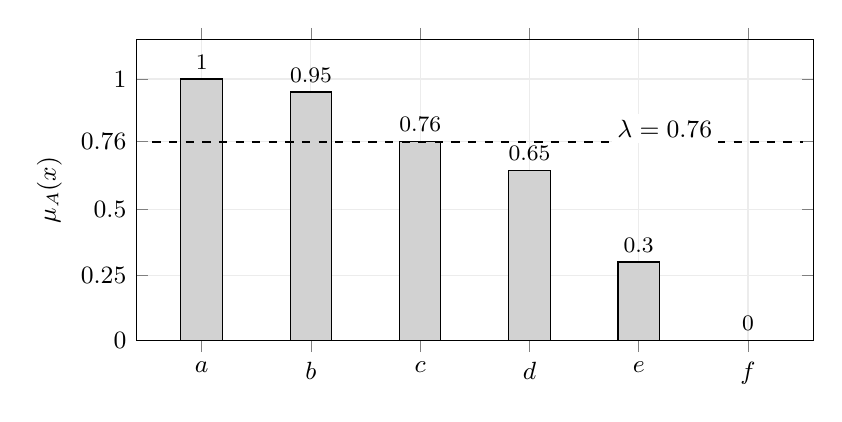
\begin{tikzpicture}
\begin{axis}[width=.84\textwidth,height=5.4cm,ybar,bar width=15pt,ymin=0,ymax=1.15,xmin=.4,xmax=6.6,xtick={1,2,3,4,5,6},xticklabels={$a$,$b$,$c$,$d$,$e$,$f$},ytick={0,.25,.5,.76,1},ylabel={$\mu_A(x)$},tick label style={font=\small},label style={font=\small},grid=major,grid style={gray!15},nodes near coords,nodes near coords style={font=\footnotesize},clip=false]
\addplot[fill=gray!35,draw=black] coordinates {(1,1)(2,.95)(3,.76)(4,.65)(5,.30)(6,0)};
\draw[dashed,thick] (axis cs:.55,.76)--(axis cs:6.5,.76);
\node[anchor=west,font=\small,fill=white,inner sep=2pt] at (axis cs:4.75,.81) {$\lambda=0.76$};
\end{axis}
\end{tikzpicture}
\caption{课程六元素实例的隶属度分布。临界元素 $c$ 属于普通截集，但不属于强截集。}
\label{fig:course}
\end{figure}

由定义可得
\begin{equation}
\cut{0.76}=\set{a,b,c},\qquad\scut{0.76}=\set{a,b}.
\eqtag{eq:course-results}
\end{equation}
临界集合只能在 $\set{a,b}$ 与 $\set{a,b,c}$ 之间选择。若 $c$ 不进入 $H(0.76)$，普通截集仍能通过所有下方集合恢复；若 $c$ 进入该集合，强截集仍通过上方并集排除它。

普通式需要排除 $d,e,f$，对应的中点见证分别为 $0.705$、$0.530$、$0.380$；强式需要找回 $a,b$，对应见证分别为 $0.880$、$0.855$。所有这些高度均严格位于目标高度的相应一侧。表~\ref{tab:witness} 列出其实际集合。

\begin{table}[htbp]
\centering\small
\caption{六元素实例在 $\lambda=0.76$ 处的中点见证证书}
\label{tab:witness}
\begin{tabular}{cccl}
\toprule
恢复方向 & 目标元素 & 见证高度 & $H(\alpha)$\\
\midrule
普通截集 & $f$ & $0.380$ & $\set{a,b,c,d}$\\
普通截集 & $e$ & $0.530$ & $\set{a,b,c,d}$\\
普通截集 & $d$ & $0.705$ & $\set{a,b,c}$\\
\midrule
强截集 & $b$ & $0.855$ & $\set{a,b}$\\
强截集 & $a$ & $0.880$ & $\set{a,b}$\\
\bottomrule
\end{tabular}
\end{table}

这些高度均不等于任何课程实例的隶属度，故其 $H$ 没有可选边界。由单阈值定理还可直接得到
\begin{equation}
H(0.705)=\cut{0.76},\qquad H(0.855)=\scut{0.76}.
\eqtag{eq:course-single}
\end{equation}
其依据是目标高度下方最近值为 $0.65$，上方最近值为 $0.95$。这一结果既与无限恢复式一致，也与逐元素有限证书一致。

\subsection{全部截集的分段表示}
六元素实例还可用于核对整个高度区间。普通与强截集分别为
\begin{equation}
\cut{\lambda}=\begin{cases}
\set{a,b,c,d,e,f},&\lambda=0,\\
\set{a,b,c,d,e},&0<\lambda\le0.30,\\
\set{a,b,c,d},&0.30<\lambda\le0.65,\\
\set{a,b,c},&0.65<\lambda\le0.76,\\
\set{a,b},&0.76<\lambda\le0.95,\\
\set{a},&0.95<\lambda\le1,
\end{cases}
\eqtag{eq:piecewise-normal}
\end{equation}
\begin{equation}
\scut{\lambda}=\begin{cases}
\set{a,b,c,d,e},&0\le\lambda<0.30,\\
\set{a,b,c,d},&0.30\le\lambda<0.65,\\
\set{a,b,c},&0.65\le\lambda<0.76,\\
\set{a,b},&0.76\le\lambda<0.95,\\
\set{a},&0.95\le\lambda<1,\\
\varnothing,&\lambda=1.
\end{cases}
\eqtag{eq:piecewise-strong}
\end{equation}
两者在每个临界高度的端点归属相反，而在相邻临界值之间相同。这样的分段表示可用于检查公式中的不等号方向，并避免将边界差异误当作数值误差。

\section{端点约定与有限采样的局限}\label{sec:endpoints}
\subsection{空索引族端点}
当 $\lambda=0$ 时，$[0,1]$ 中没有满足 $\alpha<0$ 的高度；当 $\lambda=1$ 时，没有满足 $\alpha>1$ 的高度。因而课程定理在普通式中排除 0，在强式中排除 1。采用集合论中的空族约定
\begin{equation}
\bigcap\varnothing=X,\qquad\bigcup\varnothing=\varnothing,
\eqtag{eq:empty}
\end{equation}
同时注意 $\cut0=X$、$\scut1=\varnothing$，两种恢复式即可延伸到全部 $\lambda\in[0,1]$。因此，端点限制反映的是索引族与约定的处理方式，并非等式在端点必然失效。

本节延伸与第 4 节使用的 $\sup_{[0,1]}\varnothing=0$ 属于不同层次的约定：前者涉及 $\Pow(X)$ 中的交并，后者涉及 $[0,1]$ 中的上确界。明确所处的完备格，可避免把实数扩展体系中的 $\sup\varnothing=-\infty$ 混用于隶属度重构。

\subsection{有限固定采样不能替代一般证明}
\begin{proposition}[有限下方采样的反例]
给定 $0<\lambda\le1$ 以及非空有限集合 $F\subset[0,\lambda)$，存在一元素模糊集与合法集合族，使 $\bigcap_{\alpha\in F}H(\alpha)\ne\cut{\lambda}$。
\end{proposition}
\begin{proof}
令 $u=\max F<\lambda$，取 $X=\set{x}$，$\muA(x)=(u+\lambda)/2$。对每个 $\alpha\in F$，都有 $\muA(x)>\alpha$，所以 $x\in H(\alpha)$；但 $\muA(x)<\lambda$，所以 $x\notin\cut{\lambda}$。可取 $H(\alpha)=\scut{\alpha}$ 为具体合法集合族。\end{proof}

类似地，对非空有限 $F\subset(\lambda,1]$，令 $v=\min F$ 并取 $\muA(x)=(\lambda+v)/2$。此时 $x$ 属于强截集，却被每个采样高度排除，因此有限并集不能恢复它。这两个反例说明，即使论域只有一个元素，预先固定且不依赖数据的有限采样也不能保证对所有模糊集精确。

更一般地，有限下方交集总是普通截集的外近似，有限上方并集总是强截集的内近似：
\begin{equation}
\cut{\lambda}\subseteq\bigcap_{\alpha\in F_-}H(\alpha),
\qquad
\bigcup_{\alpha\in F_+}H(\alpha)\subseteq\scut{\lambda}.
\eqtag{eq:sample-bound}
\end{equation}
其中 $F_-$ 只取下方高度，$F_+$ 只取上方高度。增加合法样本会使前者缩小、后者扩大，但是否已精确仍需见证条件或相邻值间隙保证。

\subsection{夹逼条件的两个方向缺一不可}
仅要求 $H(\alpha)\subseteq\cut{\alpha}$ 不足以保证恢复：取 $X=\set{x}$、$\muA(x)=0.60$、$H(\alpha)=\varnothing$，该上界对所有高度成立，但普通 $0.60$ 截集非空，而下方交集为空。仅要求 $\scut{\alpha}\subseteq H(\alpha)$ 也不足够：取相同模糊集且 $H(\alpha)=X$，则下界成立，但强 $0.60$ 截集为空，而上方并集为 $X$。

证明中的两项夹逼条件承担不同任务。下界保证严格高于索引高度的元素不会丢失，上界保证严格低于索引高度的元素不会被误加入。中点把待判定元素放到严格不等式的一侧，才能利用这两项保证。

\section{离散计算与可复核验证}
\subsection{边界比较的精确编码}
对应的交互讲义和演示项目\cite{project}采用千分单位整数表示课程数据：例如 $0.76$ 编码为 760，$0.95$ 编码为 950。截集与 $H$ 的成员资格直接通过整数上的 $>$、$\ge$、$=$ 比较得到，避免通过误差容忍量改变数学定义。

若中点的编码为半整数，例如 $(760+761)/2=760.5$，其真实高度为 $0.7605$。半整数可由二进制浮点数精确表示；展示时必须保留足够小数位，不能将 $0.7605$ 四舍五入回 $0.760$ 后再用于判断。整数编码的精确性依赖输入本来就在相应网格上；对于一般实数数据，量化本身可能改变边界关系。

\subsection{验证范围与结果}
项目中的数学检查枚举四元素实例的 $2^4=16$ 种边界选择和六元素实例的 $2^6=64$ 种边界选择。每个元素的选择在其自身临界高度生效。对每种选择，取 $\lambda=k/1000$，$k=0,\ldots,1000$，分别检查左右有限证书与直接截集计算是否一致。

两组数据的总恢复检查数为
\begin{equation}
(16+64)\times1001\times2=160\,160.
\eqtag{eq:case-count}
\end{equation}
全部检查通过。此外，项目检查见证严格位于相应开区间、集合族在临界高度及相邻高度处单调，以及六元素目标结果和空族约定。针对单阈值压缩结论，在相同边界枚举与阈值网格下另行执行 160160 组检查，也全部通过；两项计数对应不同的验证过程，不能作为不同数据规模相加。验证方法见附录。

\begin{table}[htbp]
\centering\small
\caption{验证设置及其证明范围}
\label{tab:validation}
\begin{tabular}{p{3.4cm}p{5.8cm}p{3.9cm}}
\toprule
检查项目 & 设置或结果 & 结论范围\\
\midrule
合法边界选择 & 四元素 16 种，六元素 64 种 & 给定实例全部选择\\
左右恢复证书 & 1001 个目标高度，共 160160 组通过 & 给定数据与离散网格\\
课程关键阈值 & 普通截集 $\set{a,b,c}$，强截集 $\set{a,b}$ & $\lambda=0.76$\\
一般截集恢复 & 四个包含方向的严格论证 & 任意论域与合法 $H$\\
有限证书压缩 & 相邻值间隙与单调性证明 & 有限隶属度值集\\
\bottomrule
\end{tabular}
\end{table}

枚举结果支持实现正确性，但没有覆盖全部实数阈值与所有可能论域。一般结论由第 3 至第 5 节的证明保证。交互动画中有限个高度的结果，应被理解为定理的可视化实例，而不是对无限集合运算的实验性证明。

\section{结论}
在普通截集与强截集之间选择合法集合族时，唯一可变部分是临界等值层。对目标高度下方的集合取交，所有隶属度达到目标高度的元素都被保留，任何较低元素都可由严格位于两者之间的中点排除；对上方集合取并，任何严格较高元素都可由中点找回，其余元素则在全部上方高度被排除。这一量词结构完整解释了两种截集的恢复。

夹逼条件同时保证集合族递减，并使其确定唯一的隶属函数。稠密高度集合或适当单侧序列可替代全部连续高度，而对于有限隶属度值集，逐元素中点证书又可压缩为位于相邻值间隙中的单一高度。上述结论在数学上区分了完整恢复、有限证书、固定采样近似和数值验证。

六元素课程实例中，$c$ 在 $H(0.76)$ 处的选择不影响普通截集 $\set{a,b,c}$ 与强截集 $\set{a,b}$。这一现象所反映的不是边界差异消失，而是边界差异可以由集合族两侧的序结构准确定位。广义分解定理因此提供了从模糊信息到清晰截集、再由清晰集合族重构隶属函数的统一数学描述。

\appendix
\section{有限证书与单阈值验证过程}
给定数据 $\set{(x_i,m_i)}_{i=1}^{n}$、目标高度 $\lambda$ 和合法的边界选择规则，以下过程可复核第 5 节的结果。
\begin{enumerate}[label=\arabic*.,leftmargin=2.4em,itemsep=3pt]
\item 直接生成基准集合 $N=\set{x_i:m_i\ge\lambda}$ 与 $S=\set{x_i:m_i>\lambda}$。
\item 对每个 $m_i<\lambda$ 取 $(m_i+\lambda)/2$，去重后计算对应 $H$ 的交集；初始交集取整个论域。
\item 对每个 $m_i>\lambda$ 取 $(m_i+\lambda)/2$，去重后计算对应 $H$ 的并集；初始并集取空集。
\item 比较两项结果与 $N,S$，并检查各见证分别满足 $m_i<\alpha<\lambda$ 或 $\lambda<\alpha<m_i$。
\item 当 $\lambda>0$ 时，使用最大较低值构造 $\gamma_-$，不存在较低值时取 $\lambda/2$；检查 $H(\gamma_-)=N$。
\item 当 $\lambda<1$ 时，使用最小较高值构造 $\gamma_+$，不存在较高值时取 $(\lambda+1)/2$；检查 $H(\gamma_+)=S$。被排除的索引端点使用空族约定。
\end{enumerate}

逐元素证书至多包含 $n$ 个高度；若逐一计算每个高度的完整成员列表，朴素实现需要 $O(n^2)$ 次比较。使用单阈值压缩，在隶属度已知时可将比较成本降为 $O(n)$。若采用排序结构并反复查询多个目标高度，相邻临界值可以通过二分定位；输出集合仍需计入成员枚举的成本。

\section{记号与课程内容对应}
\begin{longtable}{p{2.7cm}p{10.2cm}}
\caption{主要记号}\label{tab:notation}\\
\toprule 记号 & 含义\\\midrule\endfirsthead
\toprule 记号 & 含义\\\midrule\endhead
$X,\Pow(X)$ & 论域及其幂集\\
$\mu_A(x)$ & 元素 $x$ 对模糊集 $A$ 的隶属度\\
$A_\lambda,A_\lambda^+$ & 普通截集与强截集，分别使用 $\ge\lambda$ 与 $>\lambda$\\
$E_\lambda,B_\lambda$ & 临界等值层及其中由 $H$ 选取的子集\\
$H(\alpha)$ & 满足强截集与普通截集夹逼条件的清晰集合\\
$\lambda,\alpha$ & 目标高度与用于恢复的索引高度，均在 $[0,1]$ 内\\
$W^-_\lambda,W^+_\lambda$ & 左右恢复的有限中点见证高度集合\\
$m_-,m_+$ & 严格低于或高于目标高度的相邻隶属度值\\
$\gamma_-,\gamma_+$ & 位于相邻值间隙中的精确重构高度\\
\bottomrule
\end{longtable}

第 2 节对应演示中的截集定义和 $H$ 的边界选择；第 3 节对应左右恢复动画与严格证明；第 6 节对应四元素教学例及课程六元素例；第 7 节对应端点说明和有限采样提醒。第 4、5 节与附录给出课堂演示之外的补充推导，用于把七分钟讲解扩展为完整的专题报告。

\begin{thebibliography}{9}
\small
\bibitem{zadeh} L. A. Zadeh. Fuzzy sets. \textit{Information and Control}, 1965, 8(3): 338--353. DOI: \href{https://doi.org/10.1016/S0019-9958(65)90241-X}{10.1016/S0019-9958(65)90241-X}.
\bibitem{klir} G. J. Klir, B. Yuan. \textit{Fuzzy Sets and Fuzzy Logic: Theory and Applications}. Upper Saddle River, NJ: Prentice Hall, 1995. ISBN: 978-0-13-101171-7.
\bibitem{zimmermann} H.-J. Zimmermann. \textit{Fuzzy Set Theory and Its Applications}. 4th ed. Dordrecht: Kluwer Academic Publishers, 2001. DOI: \href{https://doi.org/10.1007/978-94-010-0646-0}{10.1007/978-94-010-0646-0}.
\bibitem{course} 那日萨. 第3章 模糊向清晰的转换. 系统数学课程讲义, 2016 年 9 月, 第 30、32--35、37、41 页.
\bibitem{project} xzwu-ui. 模糊集广义分解定理交互讲义与课堂演示. GitHub 源码仓库, 提交版本 7d23f53, 2026. \url{https://github.com/xzwu-ui/fuzzy-decomposition-slides}. 访问日期: 2026-10-13.
\end{thebibliography}
\end{document}
